\documentclass[tikz,border=10pt]{standalone}
\usepackage[T1]{fontenc}
\usepackage{lmodern}
\usepackage{tikz}
\usetikzlibrary{arrows.meta,calc,decorations.pathreplacing,fit,matrix,positioning}

\definecolor{cornellred}{HTML}{B31B1B}
\definecolor{ink}{HTML}{202124}
\definecolor{muted}{HTML}{667085}
\definecolor{line}{HTML}{AEB8C6}
\definecolor{paper}{HTML}{FFFFFF}
\definecolor{soft}{HTML}{F5F7FA}
\definecolor{camera}{HTML}{E8F4FF}
\definecolor{memory}{HTML}{F0F7EC}
\definecolor{compute}{HTML}{FFF3E6}
\definecolor{display}{HTML}{F7ECF3}
\definecolor{verify}{HTML}{EFEAFE}

\tikzset{
  font=\sffamily,
  flow/.style={
    -{Latex[length=2.6mm,width=1.8mm]},
    draw=muted,
    line width=0.8pt,
    rounded corners=2pt
  },
  dataflow/.style={
    flow,
    draw=cornellred
  },
  block/.style={
    rectangle,
    rounded corners=3pt,
    draw=line,
    line width=0.8pt,
    fill=paper,
    align=center,
    minimum width=28mm,
    minimum height=10mm,
    inner xsep=4pt,
    inner ysep=4pt
  },
  smallblock/.style={
    block,
    minimum width=22mm,
    minimum height=8mm,
    font=\sffamily\scriptsize
  },
  title/.style={
    font=\sffamily\bfseries\large,
    text=ink
  },
  labeltext/.style={
    font=\sffamily\scriptsize,
    text=muted,
    align=center
  },
  camera_block/.style={block, fill=camera, draw=blue!45!black},
  memory_block/.style={block, fill=memory, draw=green!45!black},
  compute_block/.style={block, fill=compute, draw=orange!65!black},
  display_block/.style={block, fill=display, draw=purple!45!black},
  verify_block/.style={block, fill=verify, draw=violet!50!black},
  groupbox/.style={
    draw=line,
    rounded corners=5pt,
    line width=0.7pt,
    fill=soft,
    inner sep=7pt
  }
}


\begin{document}
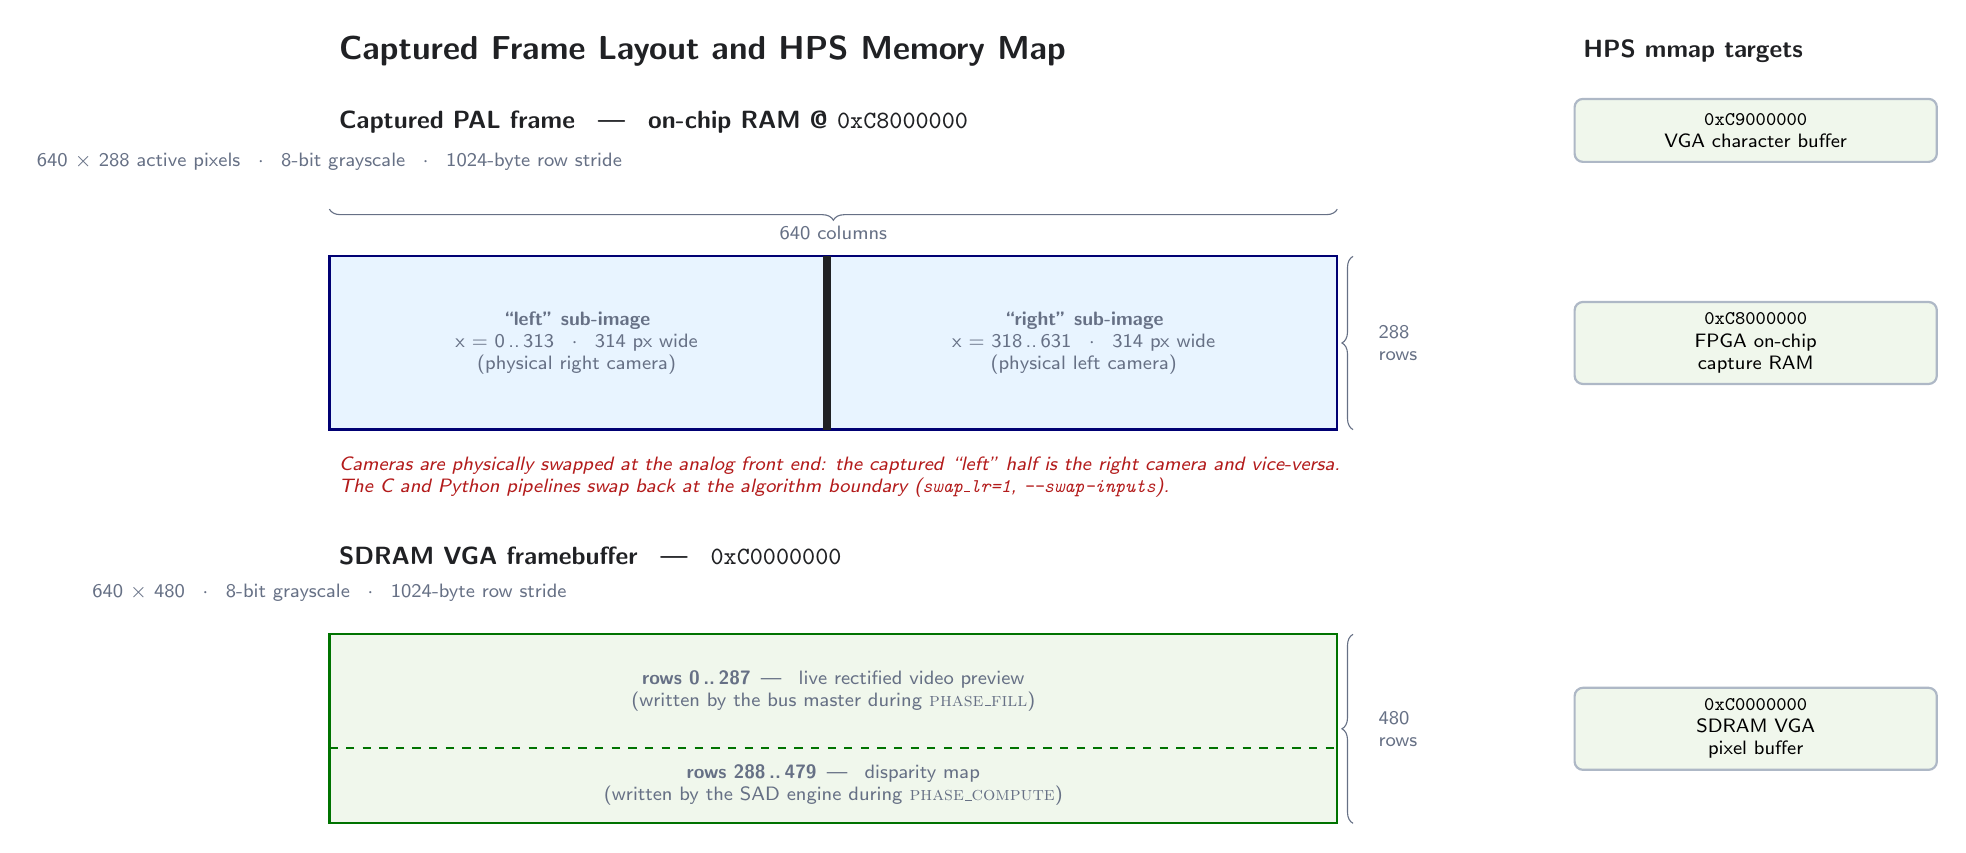
\begin{tikzpicture}[x=1mm,y=1mm]

  % ============================================================
  % Title
  % ============================================================
  \node[title, anchor=west] at (0, 96)
    {Captured Frame Layout and HPS Memory Map};

  % ============================================================
  % PANEL 1 — Captured PAL frame in FPGA on-chip RAM
  % ============================================================
  \node[font=\sffamily\small\bfseries, text=ink, anchor=west] (cap_hdr)
       at (0, 87)
       {Captured PAL frame \, --- \, on-chip RAM @ \texttt{0xC8000000}};
  \node[labeltext, anchor=west, below=0mm of cap_hdr.south west]
       (cap_sub)
       {640 $\times$ 288 active pixels \, $\cdot$ \, 8-bit grayscale \, $\cdot$ \, 1024-byte row stride};

  % Top "640 columns" brace
  \draw[decorate, decoration={brace, amplitude=4pt, mirror}, draw=muted]
       (0, 76) -- (128, 76);
  \node[labeltext] at (64, 73) {640 columns};

  % The frame rectangle (the dark bar at x=314..317 is drawn in the middle)
  \draw[fill=camera, draw=blue!45!black, line width=0.8pt]
       (0, 48) rectangle (128, 70);
  \draw[fill=ink, draw=ink]
       (62.8, 48) rectangle (63.6, 70);

  % Sub-image labels inside each half
  \node[labeltext, align=center] at (31.4, 59)
       {\textbf{``left'' sub-image}\\
        x = 0\,..\,313 \, $\cdot$ \, 314 px wide\\
        (physical right camera)};
  \node[labeltext, align=center] at (95.8, 59)
       {\textbf{``right'' sub-image}\\
        x = 318\,..\,631 \, $\cdot$ \, 314 px wide\\
        (physical left camera)};

  % Right-side "288 rows" brace
  \draw[decorate, decoration={brace, amplitude=4pt}, draw=muted]
       (130, 48) -- (130, 70);
  \node[labeltext, anchor=west, align=left] at (132, 59) {288\\rows};

  % Cameras-swapped note in cornellred so it pops as a "watch out"
  \node[labeltext, anchor=west, align=left, text=cornellred,
        font=\sffamily\scriptsize\itshape]
       at (0, 42)
       {Cameras are physically swapped at the analog front end:
        the captured ``left'' half is the right camera and vice-versa.\\
        The C and Python pipelines swap back at the algorithm boundary
        (\texttt{swap\_lr=1}, \texttt{--swap-inputs}).};

  % ============================================================
  % PANEL 2 — SDRAM VGA framebuffer (top half: preview, bottom: disparity)
  % ============================================================
  \node[font=\sffamily\small\bfseries, text=ink, anchor=west] (vga_hdr)
       at (0, 32)
       {SDRAM VGA framebuffer \, --- \, \texttt{0xC0000000}};
  \node[labeltext, anchor=west, below=0mm of vga_hdr.south west]
       (vga_sub)
       {640 $\times$ 480 \, $\cdot$ \, 8-bit grayscale \, $\cdot$ \, 1024-byte row stride};

  % VGA buffer block; 480 rows mapped to 24 mm height, so the row=288
  % boundary lives at  22 - (288/480)*24 = 22 - 14.4 = 7.6 from the bottom...
  % We draw bottom at y=-2 and top at y=22 (24 mm tall). The 288/480 cut
  % from the TOP is 14.4 mm down  ->  y = 22 - 14.4 = 7.6.
  \draw[fill=memory, draw=green!45!black, line width=0.8pt]
       (0, -2) rectangle (128, 22);
  \draw[draw=green!45!black, line width=0.6pt, dashed]
       (0, 7.6) -- (128, 7.6);

  \node[labeltext, align=center] at (64, 14.8)
       {\textbf{rows 0\,..\,287}\, --- \, live rectified video preview\\
        (written by the bus master during \textsc{phase\_fill})};
  \node[labeltext, align=center] at (64, 2.8)
       {\textbf{rows 288\,..\,479}\, --- \, disparity map\\
        (written by the SAD engine during \textsc{phase\_compute})};

  % Right-side "480 rows" brace. The boundary between the two halves
  % is already obvious from the dashed divider and the row labels, so
  % no separate "row 288" callout is needed.
  \draw[decorate, decoration={brace, amplitude=4pt}, draw=muted]
       (130, -2) -- (130, 22);
  \node[labeltext, anchor=west, align=left] at (132, 10) {480\\rows};

  % ============================================================
  % PANEL 3 — HPS memory-map reference column (right side)
  %
  % Vertically aligned with the panel each address owns: the on-chip
  % capture RAM block sits at the y of the captured-frame panel; the
  % SDRAM pixel buffer block sits at the y of the VGA buffer panel.
  % The character buffer is unrelated to either panel so it floats
  % at the top of the column. The addresses are already repeated in
  % the panel headers, so no leader arrows are needed — the spatial
  % alignment is the cue.
  % ============================================================
  \node[font=\sffamily\small\bfseries, text=ink, anchor=west] (mmap_hdr)
       at (158, 96)
       {HPS mmap targets};

  \node[smallblock, minimum width=46mm, anchor=west, fill=memory]
       (mb_chr) at (158, 86)
       {\texttt{0xC9000000}\\VGA character buffer};

  \node[smallblock, minimum width=46mm, anchor=west, fill=memory]
       (mb_cap) at (158, 59)
       {\texttt{0xC8000000}\\FPGA on-chip\\capture RAM};

  \node[smallblock, minimum width=46mm, anchor=west, fill=memory]
       (mb_vga) at (158, 10)
       {\texttt{0xC0000000}\\SDRAM VGA\\pixel buffer};

\end{tikzpicture}
\end{document}
